% !TeX root = ../thuthesis-example.tex

\chapter{树状区块链的出租车调度系统测试}

\section{实验说明}

前文中提到,现有的树状区块链添加了geohash编码的地理位置属性,提供了区域搜索的功能,本章实验就是测试现有的树状区块链在实际的出租车调度应用中的表现。

以第三章所描述的树状区块链的复现实验为基础,构建基于实际地理位置的多链区块链,并运行出租车调度系统,通过设定好乘客和车辆的初始账户数目后进行实验,统计乘客端和司机端在运行整个调度系统中所消耗的时间并将其可视化。测试树状多链区块链多链同时运行相较于单链运行的对于机器性能的负载要求。

同时,笔者还对现有仓库中的测试脚本进行了修改与重构,并提供了详细的操作说明,简化了部分操作,提高了代码的复用性,也方便后续工作者的进一步的实验。

\section{实验设计介绍}

在本章实验中,树状区块链的构成为一条虚拟父链,对应的地理位置为真实世界地图中Geohash编码前缀为wx4e的区域,其下有4条子链,对应的地理位置分别为Geohash编码前缀为wx4en、wx4ep、wx4eq和wx4er的4个区域。笔者在每条链中均分配了多位司机和乘客账户,所有司机的初始位置均相同,所有乘客之间的出发地点和目的地也相同。以上地点的选点工作基于蒙思洁完成的真实地图信息提取与筛选工作进行,已提前确保选择的路线可以在真实世界地图上导航成功。

本章实验主要使用JavaScript脚本来模拟司乘交互的整个过程。具体流程如图\ref{fig:出租车调度系统的运行流程图}所示。总体来说,司机端模拟脚本负责将司机的公钥地址,初始位置上传到区块链上,之后,便是监听一系列与乘客交互的合约中定义的事件,最终按顺序完成接单,导航,确认完成订单这一系列行为。乘客端的模拟脚本负责将乘客的公钥地址,起点位置和目的位置上传到区块链上,之后每隔一段时间将有一名乘客提交乘车请求,并搜索周围车辆账户,选取离乘客出发点曼哈顿距离最近的车辆账户相应匹配,尝试建立连接;若车辆目前已被占用,则等待一段时间后,继续重复上述操作。在乘客与车辆建立连接后,便是调用一系列合约中的事件函数进行交互,最终按顺序完成上车,到达目的地付款,确认完成订单这一系列行为。

\begin{figure}
	\centering
	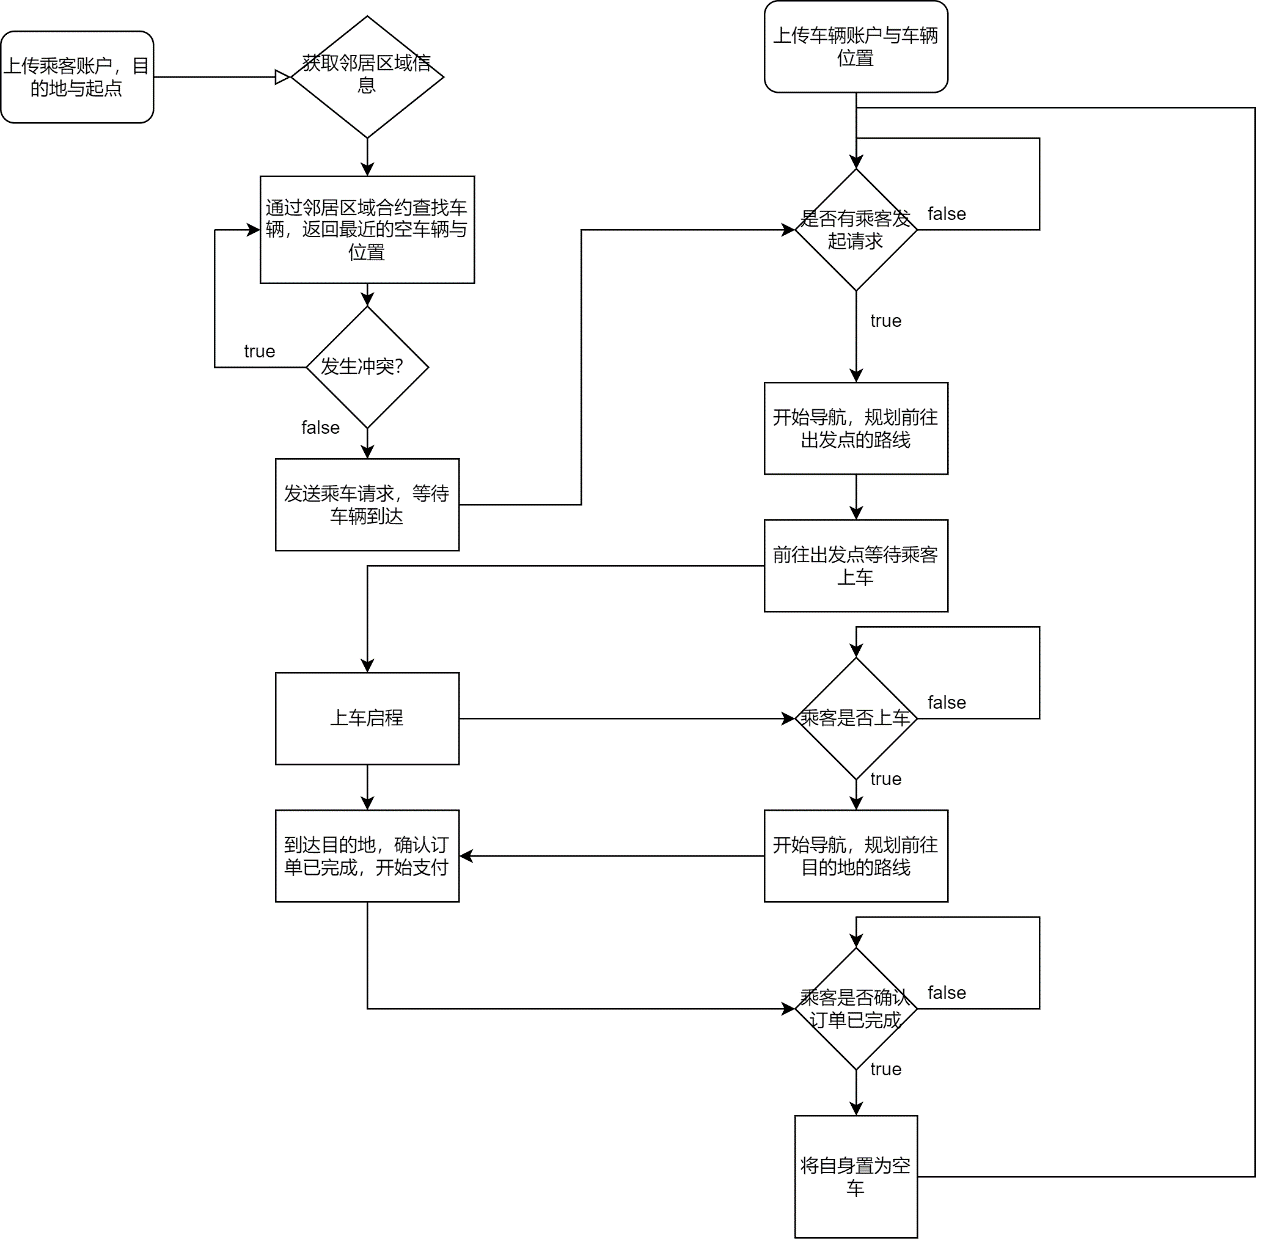
\includegraphics[width=\textwidth]{figures/出租车调度系统的运行流程图.png}
	\caption{出租车调度系统的运行流程图}
	\label{fig:出租车调度系统的运行流程图}
\end{figure}

\section{实验数据设计}

本实验的一个重点便是在于乘客与司机的初始位置的确立。实验中在4条链的区域内,各选择了一条能够进行双向导航的路径,并把该路径的起点作为乘客的起点,终点作为乘客的目的地,司机的初始位置则设为了乘客的目的地,即该路径的终点。这样在运行调度系统时,车辆先完成一次由路径终端到路径始端的导航,接到乘客后,车辆就再完成一次由路径始端到路径终端的导航。经多次实验测试,最终挑选了如表4-1中的点位数据来进行本章实验。

\begin{table}[htbp]
    \linespread{1.5}
    \zihao{5}
    \centering
    \caption{测试数据集选点}\label{测试数据集选点}
    \begin{tabular}{c|c|c|c} \toprule
        区域Geohash前缀 & 乘客起点        & 乘客终点        & 司机初始位置      \\\hline
        wx4en       & wx4enscgue5 & wx4enrq9mm9 & wx4enrq9mm9 \\
        wx4ep       & wx4epb8scg1 & wx4ep8e5gw0 & wx4ep8e5gw0 \\
        wx4eq       & wx4eq7rgmxk & wx4eqt6u0vu & wx4eqt6u0vu \\
        wx4er       & wx4erd4xkyz & wx4erw9rmze & wx4erw9rmze \\
        \bottomrule
    \end{tabular}
\end{table}

在链中初始化账户信息,并将其按照1:2的比例分为车辆账户与乘客账户,在本次实验中,参与测试的账号共有48个。其中车辆账户16个,每条链中分配4个,乘客账户32个,每条链中分配8个。划分方式,将eth.accounts中管理员外的账户,平均分配到了四条子链做当前链的活跃账户。

仓库中存有快捷分配账户的脚本,此外,分配到各链当中的信息也会以JSON格式存储到本地文件当中,便于后续查看账户具体信息和脚本读取所用。

\section{进行多子链的实验测试}

\subsection{编译并配置树状区块链}

下载实现的树状区块链的源码之后,配置好需要的编译环境,之后在源代码目录终端输入make geth,待编译完成后可以在build/bin目录中找到生成的geth可执行文件,在此实验中,将其重命名为了geth-tree后复制到了/usr/local/bin目录中,此后便可通过geth-tree指令来建立并启动区块链。

\subsection{进行实验}

本节实验的测试代码以及详细的操作文档均收录在本人的毕设仓库中,因此,本节主要介绍一下实验的大体过程。

\subsubsection{四子链并行实验}

\begin{enumerate}
    \item 准备测试用的司乘数据,运行脚本自动执行账户划分工作,结果存于仓库中的json格式的文件中
    \item 按照操作顺序启动四条子链,构建四子链网络,注意此步骤需要确保四个子链中./gethdata/keystore文件夹下均拥有相同的48个账号,并且账号均处于解锁状态(可以运行脚本自动操作)
    \item 在四子链上分别部署合约,并在乘客端和司机端的测试脚本中更新合约地址
    \item 上传地图文件
    \item 依次启动四条子链开始挖矿,同时运行乘客端和司机端的测试脚本,等待测试结束
    \item 对得到的输出文件进行可视化处理
\end{enumerate}

\subsubsection{四子链分别进行单独的单链实验}

对四条子链均分别进行单独的单链测试并取四条链结果的平均值。分别测试单链中含有12个账户(4个司机8个乘客)时,平均每个订单,乘客端与司机端所消耗的时间。

\section{结果分析}

本章测试分别统计了车辆端与乘客端的时间戳,实验结束后,从输出的文档中获取上述的耗时数据,对其进行计算和可视化的处理,其可视化结果如图\ref{fig:乘客端平均每个账户单次调度的耗时},\ref{fig:车辆端平均每个账户单次调度的耗时}所示。图中,展示了四子链并行运行和分别运行四条子链的平均值的测试结果。

\begin{figure}
	\centering
	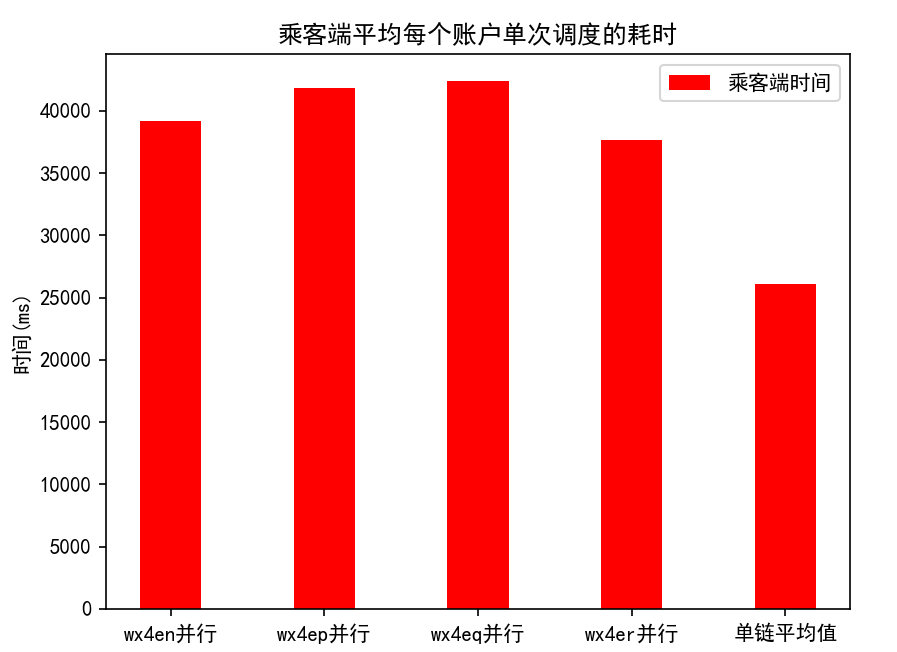
\includegraphics[width=\textwidth]{figures/乘客端平均每个账户单次调度的耗时.png}
	\caption{乘客端平均每个账户单次调度的耗时}
	\label{fig:乘客端平均每个账户单次调度的耗时}
\end{figure}

\begin{figure}
	\centering
	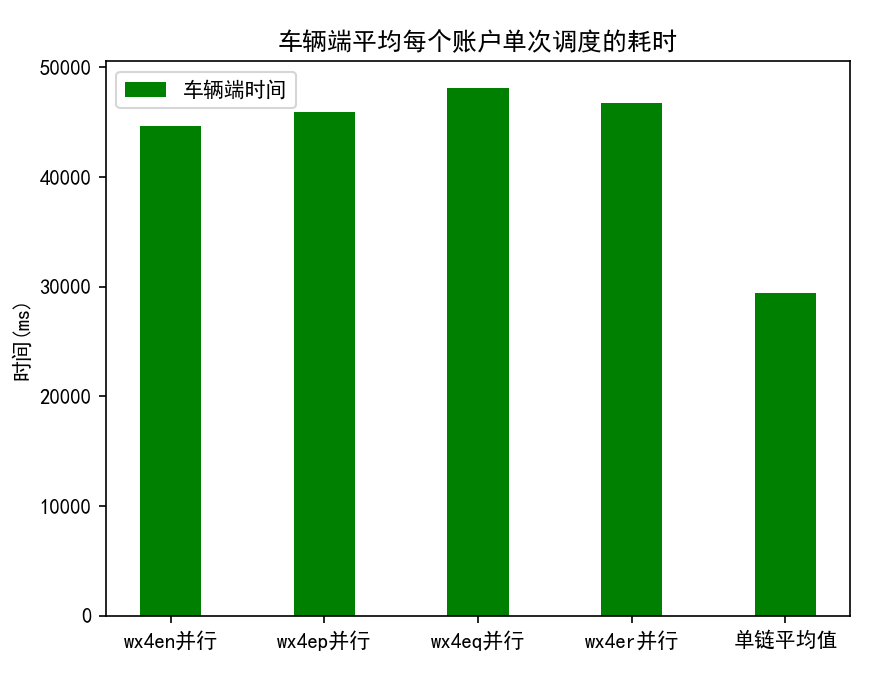
\includegraphics[width=\textwidth]{figures/车辆端平均每个账户单次调度的耗时.png}
	\caption{车辆端平均每个账户单次调度的耗时}
	\label{fig:车辆端平均每个账户单次调度的耗时}
\end{figure}

分析图中结果可以看出,虽然平均单次调度的耗时相较于单链时增多,但是若考虑是单个链中的48个账户(16个司机与32个乘客账户)的情况时,树状区块链的总耗时要远小于单链结构的情况,证实了树状区块链在车联网应用中有着良好的前景。

此外,从另一方面来看,四条子链可以并行运行出租车调度系统,但是其多链同时运行所产生的开销,也会制约树状区块链的综合性能,在后续的应用中,需要充分考虑机器的硬件配置、网络带宽、存储能力等方面,以确保系统的稳定性和安全性。

\section{本章小结}

本章主要介绍了树状多链区块链应用到出租车调度系统上的测试实验。首先,阐述了实验的设计思路;之后,以流程图的形式给出了实验的大致流程,并通过javascript脚本来模拟乘客端与车辆端的交互行为;然后是实验数据的确立,经测试选出了可以进行双向导航的测试节点,并在四条测试子链中部署了相同数目的车辆与乘客账户。接着,本章给出了实验的大致操作流程,并对结果进行了一定的分析讨论,证明了树状区块链的结构的优越,但同时也注意到为了确保系统的稳定高效,需要机器的硬件配置、网络带宽、存储能力等方面有较为优秀的配置。

